
\documentclass[11pt]{article}% use option titlepage to get the title on a page of its own.
\usepackage{blindtext}
\title{Notes on a 2-Layer Feed Forward Neural Network for Regression Tasks}
\date{2019\\ January}
\author{Jonathan Navarrete}

\usepackage{graphicx}
\usepackage{mathtools}
\usepackage{amssymb}
\usepackage{lipsum}



\begin{document}
\maketitle

\section{Introduction}
	The following notes relate to a simple feed forward neural network trained for regression tasks. The neural network has an input layer (the inputs) and two hidden layers. The first hidden layer recieves the input data and transforms it into a nonlinear space. The data is feed forward into the second hidden layer for the output. The neural network is trained using vanilla stochastic gradient descent (SGD).
	
	The neural network is implemented in a Python script (nnet.py).
	
	
\section{Architecture}

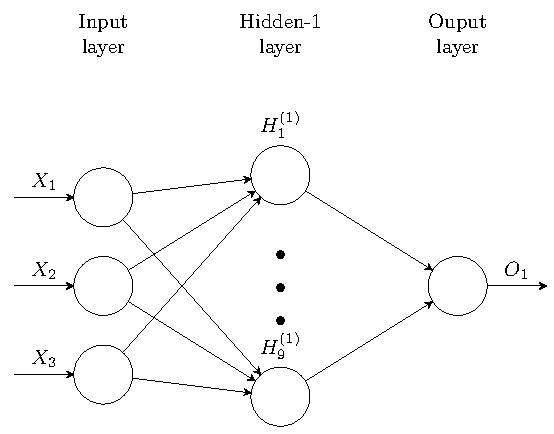
\includegraphics{nnet.pdf}

\subsection{Data}

	The neural network takes 3 inputs, where the design matrix $\mathbf{X}$ is $N \times 3$ ; however, this can be generalized to any number of $M$ inputs for a  $N \times M$ design matrix. The neural network is then fed one observation at a time, $\mathbf{x}^\intercal_i$ for $i = 1, 2, ..., N$
	
	$$
	\mathbf{X} = \begin{bmatrix}
	x_{11} & x_{12} & x_{13} \\
	x_{21} & x_{22} & x_{23} \\
	 & \cdots & \\
	x_{N1} & x_{N2} & x_{N3} \\
	\end{bmatrix} = 
	\begin{bmatrix}
	\mathbf{x}^\intercal_1 \\
	\mathbf{x}^\intercal_2 \\
	 \cdots \\
	\mathbf{x}^\intercal_N \\
	\end{bmatrix}
	$$

	There is one output target 
	$$
	\mathbf{y} = \begin{bmatrix}
	y_1 \\
	y_2 \\
 	 \cdots \\
 	y_N \\
	\end{bmatrix}
	$$
	

\subsection{First Hidden Layer}

	In the first hidden layer there are 9 hidden units $H^{(1)}_1, H^{(1)}_2, ..., H^{(1)}_9$. Each hidden unit sees each of the three 3 inputs, aggregates the inputs with weights and passes that hidden output to an activation function. The activation function used in the first hidden layer is logistic,
	
	$$
	H^{(1)}_k = f(z) = \frac{1}{1 + e^{-z}}
	$$
	
	where $z = w^{(1)}_1 x_i1 + w^{(1)}_2 x_i2 + w^{(1)}_3 x_i3$.
	
	For each hidden unit, we have three weights $\mathbf{w}^{(1)}$

\subsection{Second Hidden Layer}

	In the second hidden layer there is 1 hidden units (the output unit). Because there is only one output, $y_i$, there is only the need for one hidden unit. 
	
	The second hidden layer expects 9 inputs from the first hidden layer. The activation function is simply the identity function $g(z) = z$, where $z = w^{(2)}_1 x_i1 + w^{(2)}_2 x_i2 + w^{(2)}_9 x_i3$.
	
	
	
\section{Feed Forward}

\subsection{Input to First Hidden Layer}

For each observation $i$, we take input $\mathbf{x}^\intercal_i$ and pass it to the first layer to each hidden unit $j$
	$$
	h_j = f(z) = \frac{1}{1 + e^{-z_j}}
	$$
	where 
	$$
	z_j = \mathbf{x}^\intercal_i \mathbf{w}^{(1)}_j 
	= \begin{bmatrix}
	x_{i1} & x_{i2} & x_{i3}
\end{bmatrix}
	\begin{bmatrix}
	w^{(1)}_1 \\
	w^{(1)}_2 \\
	w^{(1)}_3 \\
	\end{bmatrix}
	= w^{(1)}_1 x_1 + w^{(1)}_2 x_2 + w^{(1)}_3 x_3 
	$$
	
	This can be more efficiently computed by using a $3 \times 9$ weights matrix 
	
	$$
	\mathbf{W}^{(1)} = \begin{bmatrix}
	\mathbf{w}^{(1)}_1 &  \mathbf{w}^{(1)}_2 & \cdots & \mathbf{w}^{(1)}_9 \\
	\end{bmatrix}
	$$
	
	Take the input row vector $\mathbf{x}^\intercal_i$ and multiply it with $W^{(1)}$ to obtain $\mathbf{z}^\intercal$
	
	$$
	\mathbf{z}^\intercal = \mathbf{x}^\intercal_i \mathbf{W}^{(1)}
	= \begin{bmatrix}
	z_1 & z_2 & \cdots & z_9
	\end{bmatrix}
	$$
	
	Afterwards, we pass the hidden layer outputs through the activation function,
	
	$$
	\mathbf{h}^\intercal = f(\mathbf{z}^\intercal)
	= \begin{bmatrix}
	h_1 & h_2 & \cdots & h_9
	\end{bmatrix}
	$$
	
	
\subsection{Hidden to Output Layer}

	After the first hidden layer is computed, the hidden outputs $\mathbf{h}^\intercal$ is fed to the output layer. The ouptut layer has 1 output and expects 9 inputs. Thus, we have a $9 \times 1$ weights matrix

	$$
	\mathbf{W}^{(2)} = \mathbf{w}^{(2)}
	= \begin{bmatrix}
	w_1 \\ 
	w_2 \\ 
	\cdots \\ 
	w_9
	\end{bmatrix}
	$$


	$$
	o_i = g(\mathbf{h^\intercal} \mathbf{w}^{(2)}) = \mathbf{h^\intercal} \mathbf{w}^{(2)}
	$$



\section{Backpropogation}


\begin{quote}
The back-propagation algorithm (Rumelhart et al., 1986a), often simply called backprop, allows the information from the cost to then flow backward throughthe network in order to compute the gradient.
[...]
The term back-propagation is often misunderstood as meaning the whole learning algorithm for multi-layer neural networks. Actually, back-propagation refers only to the method for computing the gradient, while another algorithm,such as stochastic gradient descent, is used to perform learning using this gradient. Furthermore, back-propagation is often misunderstood as being specific to multi-layer neural networks, but in principle it can compute derivatives of any function (for some functions, the correct response is to report that the derivative of the function is undefined).\footnote{https://www.deeplearningbook.org/contents/mlp.html}
\end{quote} 


\subsection{Calculation Errors}

For this regression task we will use the mean squared error (MSE) as the statistic to measure performance. We'd like to create a neural network that has a small as possible MSE. Thus we are trying to minimize MSE with respect to the weights in the neural network.

$$
MSE = \frac{1}{N} \sum^N_{i = 1} (o_i - y_i)^2 = \frac{1}{N} \sum^N_{i = 1} e_i^2 
$$

To train the neural network, it'll be necessary to differentiate this error response with respect to each weight. This will be accomplished using the backpropogation algorithm.


\subsection{Gradient for Output Layer}

	Using the backprop algorithm we will take the derivative of MSE with respect to (wrt) the weights in the output layer. Let $E = MSE(w^{(2)})$, then by the chain rule we obtain

	$$
	\frac{dE}{dw^{(2)}_k} = \frac{dE}{do_i} \frac{do_i}{dw^{(2)}_k}
	$$

	The derivative of $E$ wrt $o_i$ is 

	$$
	\frac{dE}{do_i} = \frac{2}{N}  \sum^N_{i}  (y_i - o_i)
	$$

	and the derivative of $o_i$ wrt $w^{(2)}_k$ is
	
	$$
	\frac{do_i}{dw^{(2)}_k} = \frac{d}{dw^{(2)}_k}(dw^{(2)}_1 h^{(1)}_1+ \cdots + w^{(2)}_k h^{(1)}_k + \cdots + + w^{(2)}_9 h^{(1)}_9) = h^{(1)}_k
	$$

	Thus, the partial derivate is 
	$$
	\frac{2}{N}  \sum^N_{i}  (y_i - o_i) \times h^{(1)}_k
	$$

However, this process will need to be continued for all weights $w^{(2)}_1, \cdots, w^{(2)}_9$. Taking partial derivatives for all weights gives us the gradient.

	$$
	\frac{dE}{dw^{(2)}_k} = \frac{dE}{do_i} \nabla o_i
	$$

where 

	$$
	\nabla o_i = \begin{bmatrix}
	\frac{do_i}{dw^{(2)}_1} \\ 
	\cdots \\ 
	\frac{do_i}{dw^{(2)}_9} \\ 
	\end{bmatrix}
	= \begin{bmatrix}
	h^{(1)}_1 \\
	\cdots \\
	h^{(1)}_9
	\end{bmatrix}
	$$







\subsection{Gradient for Hidden Layer}













\end{document}
